\chapter{Технологический раздел}
\label{cha:impl}


\section{Выбор операционной системы}
Выбор стоял только между дистрибутивами Linux, так как ключевой компонент разработки - фреймворк DPDK - не работает под управлением ОС семейства Windows. Критерии выбора:
\begin{itemize}
\item бесплатное распространение;
\item наличие менеджера пакетов, позволяющего устанавливать необходимое ПО из репозиториев;
\item простота настройки и конфигурирования необходимых компонент;
\end{itemize}

В качестве ОС для разработки и развертывания была выбрана ОС Ubuntu 14.04 Trusty, версия ядра 3.16.0-53-generic, так как она удовлетворяет всем критериям.


\section{Выбор языка программирования}
В качестве языка программирования для разработки был выбран C++, версия стандарта 11. Причины решения в пользу этого языка:
\begin{itemize}
\item DPDK написан на языке C;
\item является компилируемым, а не интерпретируемым языком;
\item высокие показатели производительности;
\item полная поддержка парадигмы ООП;
\item простота работы на низком уровне (битовые операции, потоки);
\item наличие бесплатных компиляторов, сред разработки;
\item наличие бесплатных фреймворков логирования и тестирования;
\item наличие бесплатных утилит отладки и профилирования;
\end{itemize}

Дополнительный плюс использования C++ - это широкие возможности стандартной библиотеки, например: контейнеры, алгоритмы, средства синхронизации. Все это пришлось бы реализовывать вручную при использовании языка C в качестве языка разработки.


\section{Другие инструменты}
\paragraph{Git}

В качестве системы управления версиями использовался git - на сегодняшний день является самым популярным и имеет самый широкий список функциональных возможностей.

В Ubuntu git можно установить из репозиториев следующей командой:
\begin{lstlisting}
sudo apt-get install git
\end{lstlisting}

В качестве удаленного хранилища был выбран github.com.

\paragraph{Vim}

Для C++ существует большое количество сред разработки, как платных, так и нет, например: QtCreator, Eclipse, Netbeans. Это сложные IDE с графическим интерфейсом, возможностью привязки системы контроля версий, встроенным отладчикам и т.д.

В качестве среды разработки данного сервиса был выбран текстовый редактор vim засчет его простоты, а также наличия в любом дистрибутиве Linux.

В Ubuntu vim можно установить из репозиториев следующей командой:
\begin{lstlisting}
sudo apt-get install vim
\end{lstlisting}

\paragraph{Latex}

В качестве инструмента разработки РПЗ использовалась система компьютерной верстки Latex. Выбор в пользу этой системы был сделан по следующим причинам:
\begin{itemize}
\item бесплатное распространение;
\item возможность верстки в любом текстовом редакторе (использовался vim);
\item развитые функциональные возможности (автоматическое оглавление, таблицы, формулы);
\item возможность хранить документ как набор отдельных .tex файлов;
\end{itemize}

В Ubuntu Latex можно установить из репозиториев следующей командой:
\begin{lstlisting}
sudo apt-get install texlive-full
\end{lstlisting}

\paragraph{Valgrind}

Для профилирования использования памяти, выходов за границы массивов и отдельных участков кода использовался valgrind. Выбор был сделан в пользу этого инструмента по следующим причинам:
\begin{itemize}
\item бесплатное распространение;
\item развитые функциональные возможности (построение временных графиков, отслеживание выходов за границы, области неинициализированных данных);
\item отслеживание утечек памяти (бесплатных аналогов нет);
\end{itemize}

В Ubuntu valgrind можно установить из репозиториев следующей командой:
\begin{lstlisting}
sudo apt-get install valgrind
\end{lstlisting}


\section{Структура приложения}
Первое действие, которое выполняется при запуске - это инициализация компонент DPDK. Ее должно выполнять любое приложение, использующее DPDK. Функция инициализации имеет следующую сигнатуру:
\begin{lstlisting}
int rte_eal_init(int argc, char *argv[]);
\end{lstlisting}

Процесс инициализации состоит из следующих частей:
\begin{itemize}
\item считывание данных с шины PCI с целью определения нужного драйвера сетевых устройств, их последующая инициализация;
\item создание нужного числа потоков, в зависимости от количества доступных ядер (используется pthread\_create);
\item привязка каждого потока к своему ядру (используется pthread\_setaffinity\_np);
\item выделение необходимого количества памяти в больших страницах (используется mmap);
\item инициализация внутренних структур и таймеров;
\end{itemize}

Далее выполняется инициализация системы логирования, для этого используется библиотека glog от компании Google. Функция инициализации имеет следующую сигнатуру:
\begin{lstlisting}
google::InitGoogleLogging(argv[0]);
\end{lstlisting}

Glog является бесплатной и может быть установлена из репозиториев Ubuntu следующей командой:
\begin{lstlisting}
sudo apt-get install libgoogle-glog-dev
\end{lstlisting}

После инициализации DPDK и системы логирования выполняется инициализация всех классов, использующихся в работе сервиса. Ниже подробно описан каждый из них.

\subsection{Класс Config}
Класс Config реализует все действия по работе с файлом конфигурации, ниже приведена его структура:
\begin{lstlisting}
class Config {
 public:
  explicit Config(const std::string &);
  ~Config();

  Config(const Config &) = delete;
  Config &operator=(const Config &) = delete;
  Config(Config &&) = delete;
  Config &operator=(Config &&) = delete;

  bool Initialize();
  void GetActions(const uint16_t, Actions *&);

 protected:
  bool ParsePortAndProtocol(uint16_t &, std::string &);
  bool ParseActions(Actions &, std::string &);
  bool ParseVlanData(uint16_t &, uint8_t &, uint8_t &, uint16_t &, std::string &);
  bool ParseMplsData(uint32_t &, uint8_t &, uint8_t &, uint8_t &, std::string &);

 private:
  std::string config_name_;
  std::unordered_map<uint16_t, Actions> rules_;
};
\end{lstlisting}

Конструктор принимает один параметр - имя файла конфигурации, которое сохраняется в член класса config\_name\_.

Метод Initialize() выполняет парсинг файла и сохраняет правила в член класса rules\_, который представлен в виде unordered\_map стандартной библиотеки C++. Этот вид контейнера выбран для быстрого поиска правил (O(1)). Ключ - 16 битное значение: первые 8 бит - номер порта, вторые 8 бит - протокол. Значением является набор действий, которые требуется применить к определенному типу трафика на определенном порту. Действия хранятся в контейнере vector стандартной библиотеки и описаны в конструкторском разделе.

Метод GetActions(...) выполняет поиск нужного правила в rules\_ по ключу, переданному первым параметром и, если поиск завершается удачно, сохраняет результат в переменную, переданную вторым параметром. В противном случае сохранется nullptr как индикатор того, что нужное правило не найдено. В этом случае трафик должен быть блокирован.

Исходный код этого класса находится в файлах config.h и config.cpp в папке src.

\subsection{Классы PortBase и PortEthernet}
Класс PortBase является абстрактным классом и используется в качестве базового для класса PortEthernet, ниже приведена его структура:
\begin{lstlisting}
class PortBase {
 public:
  explicit PortBase(const uint8_t);
  virtual ~PortBase() = default;

  PortBase(const PortBase &) = delete;
  PortBase &operator=(const PortBase &) = delete;
  PortBase(PortBase &&) = delete;
  PortBase &operator=(PortBase &&) = delete;

  virtual void SendOnePacket(rte_mbuf *, PortQueue *) = 0;
  virtual void SendAllPackets(PortQueue *) = 0;
  virtual void ReceivePackets(PortQueue *) = 0;
  uint8_t GetPortId() const;

 private:
  uint8_t port_id_;
};
\end{lstlisting}

Конструктор принимает один параметр - номер порта, который сохраняется в член класса port\_id\_.

Абстрактные виртуальные методы SendOnePacket(...), SendAllPackets(...) и ReceivePackets(...) реализуют логику отправки и приема пакетов на сетевом интерфейсе. Должны быть переопределены производными классами в соответствие с логикой их работы.

Так класс PortEthernet переопределяет эти методы для работы с Ethernet портами. Ниже приведены сигнатуры функций, которые используются для отправки и приема непосредственно на самом сетевом устройстве:
\begin{lstlisting}
uint16_t rte_eth_tx_burst(uint8_t port_id, uint16_t queue_id, rte_mbuf **tx_pkts, uint16_t nb_pkts);
uint16_t rte_eth_rx_burst(uint8_t port_id, uint16_t queue_id, rte_mbuf **rx_pkts, uint16_t nb_pkts);
\end{lstlisting}

Исходный код обоих классов находится в файлах port.h и port.cpp в папке src.

\subsection{Класс PortManager}
Класс PortManager отвечает за инициализацию сетевых интерфейсов, маппинг ядер и портов, инициализацию экземпляров PortEthernet. Ниже приведена его структура:
\begin{lstlisting}

class PortManager {
 public:
  PortManager();
  ~PortManager();

  PortManager(const PortManager &) = delete;
  PortManager &operator=(const PortManager &) = delete;
  PortManager(PortManager &&) = delete;
  PortManager &operator=(PortManager &&) = delete;

  bool Initialize();
  PortBase *GetPortByCore(const unsigned) const;
  PortBase *GetPortByIndex(const uint8_t) const;
  PortQueue *GetPortTxQueue(const unsigned, const uint8_t);
  unsigned GetStatsLcoreId() const;
  rte_mbuf *CopyMbuf(rte_mbuf *) const;

 protected:
  bool InitializePort(const uint8_t, const unsigned) const;
  void CheckPortsLinkStatus(const uint8_t) const;

 private:
  std::unordered_map<unsigned, rte_mempool *> mempools_; // socket->mempool
  std::unordered_map<unsigned, PortBase *> ports_map_;   // lcore->port
  std::vector<PortBase *> ports_;                        // ports
  PortQueue port_tx_table_[RTE_MAX_LCORE][RTE_MAX_ETHPORTS];
  unsigned stats_lcore_id_;
};
\end{lstlisting}

Метод Initialize() является ключевым и выполняет следующие действия:
\begin{itemize}
\item находит каждому порту свободное ядро, на котором этот порт будет обрабатываться, сохраняет полученное отображения в член класса ports\_map\_, который реализован в виде unordered\_map. Ключ - 4 байта, является идентификатором ядра, значение - экземпляр класса PortEthernet.
\item для каждого процессора создает rte\_mempool и сохраняет это отображение в mempools\_, реализованный в виде unordered\_map. Ключ - 4 байта, является идентификатором процессора, значение - rte\_mempool. Для создания пула памяти используется функция:
\begin{lstlisting}
rte_mempool *rte_pktmbuf_pool_create(const char *name, unsigned n, unsigned cache_size, uint16_t priv_size, uint16_t data_room_size, int socket_id);
\end{lstlisting}
\item инициализирует все сетевые порты, что подразумевает инициализацию входной и выходной очередей, запуск сетевого интерфейса, перевод его в неразборчивый режим (promiscuous mode), проверку состояния (link up/down). Для этого используется следующий набор функций:
\begin{lstlisting}
int rte_eth_dev_configure(uint8_t port_id, uint16_t nb_rx_queue, uint16_t nb_tx_queue, rte_eth_conf *eth_conf);
int rte_eth_rx_queue_setup(uint8_t port_id, uint16_t rx_queue_id, uint16_t nb_rx_desc, unsigned int socket_id, const rte_eth_rxconf *rx_conf, rte_mempool *mp);
int rte_eth_tx_queue_setup(uint8_t port_id, uint16_t tx_queue_id, uint16_t nb_tx_desc, unsigned int socket_id, const rte_eth_rxconf *tx_conf);
int rte_eth_dev_start(uint8_t port_id);
void rte_eth_link_get_nowait(uint8_t port_id, rte_eth_link *link);
\end{lstlisting}
\end{itemize}

Методы GetPortByCore(...) и GetPortByIndex(...) возвращают указатель на экземпляр PortEthernet по идентификатору ядра или номеру порта соответственно.

Член класса port\_tx\_table\_ используется для реализации выходного буфера, описанного в конструкторском разделе, а stats\_lcore\_id\_ - для хранения идентификатора ядра, на котором производится печать статистики.

Исходный код класса PortManager находится в файлах port\_manager.h и port\_manager.cpp в папке src. Там же определены значения некоторых переменных, требуемых для инициализации сетевых интерфейсов и пулов памяти.

\subsection{Класс PacketAnalyzer}
Класс PacketAnalyzer реализует логику DPI, его структура приведена ниже:
\begin{lstlisting}
class PacketAnalyzer {
 using SearchMethod = std::function<protocol_type(rte_mbuf *)>;

 public:
  PacketAnalyzer();
  ~PacketAnalyzer() = default;

  PacketAnalyzer(const PacketAnalyzer &) = delete;
  PacketAnalyzer &operator=(const PacketAnalyzer &) = delete;
  PacketAnalyzer(PacketAnalyzer &&) = delete;
  PacketAnalyzer &operator=(PacketAnalyzer &&) = delete;

  static PacketAnalyzer &Instance();
  protocol_type Analyze(rte_mbuf *) const;

 private:
  std::vector<SearchMethod> methods_;
};
\end{lstlisting}

Единственным членом класса является methods\_ - vector, состоящий из методов поиска. Каждый метод - это отдельный модуль на C++, реализующий детектирование конкретного протокола. Все модули располагаются в папке src/protocols и используются в PacketAnalyzer.

Метод Analyze(...) обрабатывает пакет каждым методом поиска из methods\_. В результате возвращается тип протокола или UNKNOWN, если не удалось отнести пакет ни к одному протоколу.

Исходный код класса PacketAnalyzer находится в файлах packet\_analyzer.h и packet\_analyzer.cpp в папке src.

\subsection{Класс PacketManager}
Класс PacketManager выполняет считывание пакетов с сетевой карты и их последующую обработку. Экземпляры классов Config и PortManager являются членами класса и используются им в процессе обработки трафика. Экземпляр PacketAnalyzer, хоть и не является членом класса PacketManager, используется для определения типа трафика. Ниже приведена структура этого класса:
\begin{lstlisting}
class PacketManager {
 public:
  PacketManager(const std::string &, const uint16_t);
  ~PacketManager() = default;

  PacketManager(const PacketManager &) = delete;
  PacketManager &operator=(const PacketManager &) = delete;
  PacketManager(PacketManager &&) = delete;
  PacketManager &operator=(PacketManager &&) = delete;

  bool Initialize();
  void RunProcessing();

 protected:
  void ProcessPackets(PortQueue *, const uint8_t);
  void ExecuteOutput(rte_mbuf *, const uint8_t);

  void PrintStats() const;

 private:
  Config config_;
  PortManager port_manager_;
  uint16_t stats_interval_;
};
\end{lstlisting}

Метод Initialize() вызывает одноименный метод у членов класса config\_ и port\_manager\_.

Метод RunProcessing() - это основной цикл обработки, именно этот метод  запускается на каждом ядре и в нем происходит вся логика работы сервиса. В зависимости от того, на каком ядре он запущен, выполняется считывание пакетов из нужного порта. Далее они обрабатываются методом ProcessPackets(...), в котором анализируются и, в зависимости от протокола, над ними выполняются действия, определенные в config\_. Также в рамках метода RunProcessing() выполняется отправка пакетов по истечению определенного интервала времени, проверка состояния порта (link up/down), подсчет и печать статистики.

Запуск основного цикла обработки выполняется после инициализации всех компонент и реализуется функцией:
\begin{lstlisting}
int rte_eal_mp_remote_launch(lcore_function_t *f, void *arg, rte_rmt_call_master_t call_master);
\end{lstlisting}

Исходный код класса PacketManager находится в файлах packet\_manager.h и packet\_manager.cpp в папке src. Запуск метода RunProcessing() производится из файла main.cpp в той же папке.

\section{Развертывание и запуск}
Для сборки и функционирования сервиса требуется установить дополнительные пакеты, сделать это можно следующей командой:
\begin{lstlisting}
sudo apt-get install g++ cmake libpcap-dev libfuse-dev
\end{lstlisting}

Далее требуется установить DPDK и настроить возможность использования больших страниц. Для этого нужно скачать архив с официального сайта~\cite{dpdk_descr} и выполнить следующие команды:
\begin{lstlisting}
sudo tar xf dpdk.tar.gz /opt/ && cd /opt/dpdk
make config T=x86_64-native-linuxapp-gcc
sed -ri 's,(PMD_PCAP=).*,\1y,' build/.config
sudo make

sudo mkdir p /mnt/huge
sudo mount -t hugetlbfs nodev /mnt/huge
sudo echo 64 > /sys/devices/system/node/node0/hugepages/hugepages-2048kB/nr_hugepages
\end{lstlisting}

На этом установка необходимых компонентов окончена и можно собрать проект, используя Cmake, следующими командами:
\begin{lstlisting}
mkdir build && cd build
cmake .. -DCMAKE_BUILD_TYPE=Release
make
\end{lstlisting}

\subsection{Аргументы командной строки}
Запуск сервиса производится из командной строки следующей командой:
\begin{lstlisting}
sudo ./dpdk_dpi -c <num_cores> -n1 -- --config <config_name> --stats-interval <seconds>
\end{lstlisting}
Ниже объясняется значение аргументов:
\begin{itemize}
\item -c <num\_cores> - используется DPDK для указания количества используемых ядер, задается в шестнадцатеричной системе счисления, обязательный;
\item --config <config\_name> - имя файла конфигурации, обязательный;
\item --stats-interval <seconds> - выводить статистику каждые seconds секунд, необязательный;
\end{itemize}

\subsection{Статистика}
Статистика собирается во время работы по каждому поддерживаемому протоколу и по общему числу полученных/отправленных пакетов. Подсчет ведется для каждого сетевого интерфейса.

Если при запуске задан ключ --stats-interval, то данные выводятся в стандартный поток вывода в следующем виде:
\begin{lstlisting}
=====Statistcics=====
port_id=0
 - Pkts in: 1
 - Pkts out: 0
     HTTP: 0
     SIP: 0
     RTP: 0
     RTSP: 0
port_id=1
 - Pkts in: 0
 - Pkts out: 0
     HTTP: 0
     SIP: 0
     RTP: 0
     RTSP: 0
====================
\end{lstlisting}


\section{Тестирование}
Процесс тестирования является неотъемлимой частью разработки любого программного обеспечения. Благодаря ему удается выявить ошибки как на уровне исходного кода, так и в функционировании всей системы.

В рамках разработки сервиса классификации трафика проводились следующие виды тестирования:
\begin{itemize}
\item Модульное;
\item Функциональное;
\item Нагрузочное;
\end{itemize}

\subsection{Модульное тестирование}
Целью модульного тестирования является изолирование отдельных частей программы и демонстрация того, что все отдельные части являются работоспособными. Обычно реализуется в виде тестирования отдельных участков кода, например методов класса, с использованием специализированного фреймворка.

В качестве фреймворка был выбран Gtest от компании Google. Он является бесплатным и может быть установлен из репозиториев Ubuntu следующей командой:
\begin{lstlisting}
sudo apt-get install libgtest-dev
cd /usr/src/gtest
sudo cmake CMakeLists.txt
sudo make
sudo cp *.a /usr/lib
\end{lstlisting}

В рамках модульного тестирования проверялись на корректность обнаружения протоколов все методы поиска. Также проводилось тестирование корректности использования аргументов командной строки.

Все тесты находятся в папке test и test/protocols. Ниже приведен фрагемнт кода для тестирования метода поиска протокола RTP:
\begin{lstlisting}
  TEST(RTP, BadExt) {
    uint8_t data[] = {
      0x00, 0x00, 0x00, 0x00, 0x00, 0x00,
      0x00, 0x00, 0x00, 0x00, 0x00, 0x00,
      0x08, 0x00,
  
      0x05, 0x00,
      0x00, 0x00,
      0x00, 0x00,
      0x00, 0x00,
      0x40, 0x11, // (ttl, proto)
      0x00, 0x00,
      0x00, 0x00, 0x00, 0x00,
      0x00, 0x00, 0x00, 0x00,
  
      0x00, 0x00,
      0x00, 0x00,
      0x00, 0x00,
      0x00, 0x00,
  
      0x90, 0x08, 0x00, 0x03,
      0x00, 0x00, 0x00, 0x00, // timestamp
      0x00, 0x00, 0x00, 0x01,
      0x00, 0x00, 0x00, 0x02,
      // ext data (second is absent)
      0x00, 0x00, 0x00, 0x00,
    };
    auto m = InitPacket(data, sizeof(data));
    ASSERT_EQ(PreparePacket(m), true);
    ASSERT_EQ(SearchRtp(m), UNKNOWN);
    rte_pktmbuf_free(m);
  }

  TEST(RTP, GoodWithoutCsrcAndWithoutExt) {
    uint8_t data[] = {
      0x00, 0x00, 0x00, 0x00, 0x00, 0x00,
      0x00, 0x00, 0x00, 0x00, 0x00, 0x00,
      0x08, 0x00,
  
      0x05, 0x00,
      0x00, 0x00,
      0x00, 0x00,
      0x00, 0x00,
      0x40, 0x11, // (ttl, proto)
      0x00, 0x00,
      0x00, 0x00, 0x00, 0x00,
      0x00, 0x00, 0x00, 0x00,
  
      0x00, 0x00,
      0x00, 0x00,
      0x00, 0x00,
      0x00, 0x00,
  
      0x80, 0x08, 0x00, 0x03,
      0x00, 0x00, 0x00, 0x00, // timestamp
      0x00, 0x00, 0x00, 0x01,
    };
    auto m = InitPacket(data, sizeof(data));
    ASSERT_EQ(PreparePacket(m), true);
    ASSERT_EQ(SearchRtp(m), RTP);
    rte_pktmbuf_free(m);
  }
\end{lstlisting}

Данный фрагмент содержит два модульных теста:
\begin{itemize}
\item в первом определяется RTP-пакет, в котором не хватает одного дополнительного заголовка, из-за чего метод поиска SearchRtp(...) возвращает UNKNOWN;
\item во втором определяется корректный RTP-пакет, поэтому SearchRtp(...) возвращает RTP;
\end{itemize}

Ниже приведены результаты запуска всех модульных тестов:
\begin{lstlisting}
[----------] Global test environment tear-down
[==========] 49 tests from 8 test cases ran. (4 ms total)
[  PASSED  ] 49 tests.
\end{lstlisting}

\subsection{Функциональное тестирование}
Целью функционального тестирования является проверка работоспособности всей системы в целом, а также корректности взаимодействия ее частей между собой.

В рамках функционального тестирования проверялась правильность определения типа трафика и выполнения действий над ним. Для этого использовались .pcap файлы, утилита tcpreplay для их "проигрывания" и утилита tcpdump для записи трафика с выходного интерфейса. Просмотр записанного на выходе файла осуществлялся с использованием Wireshark.

Все .pcap файлы для тестирования находятся в папке pcap. Wireshark можно бесплатно загрузить с официального сайта и установить на компьютере. Tcpdump уже установлен в Ubuntu 14.04, а tcpreplay устанавливается следующей командой:
\begin{lstlisting}
sudo apt-get install tcpreplay
\end{lstlisting}

На рисунке~\ref{pic:wireshark} показано содержимое файла, записанного на выходе, когда на входе используется файл HTTP.pcap и файл конфигурации с единственным правилом:
\begin{center}
1,HTT : PUSH-VLAN(33024,2,0,100);OUTPUT(2);
\end{center}

\begin{figure}
\centering
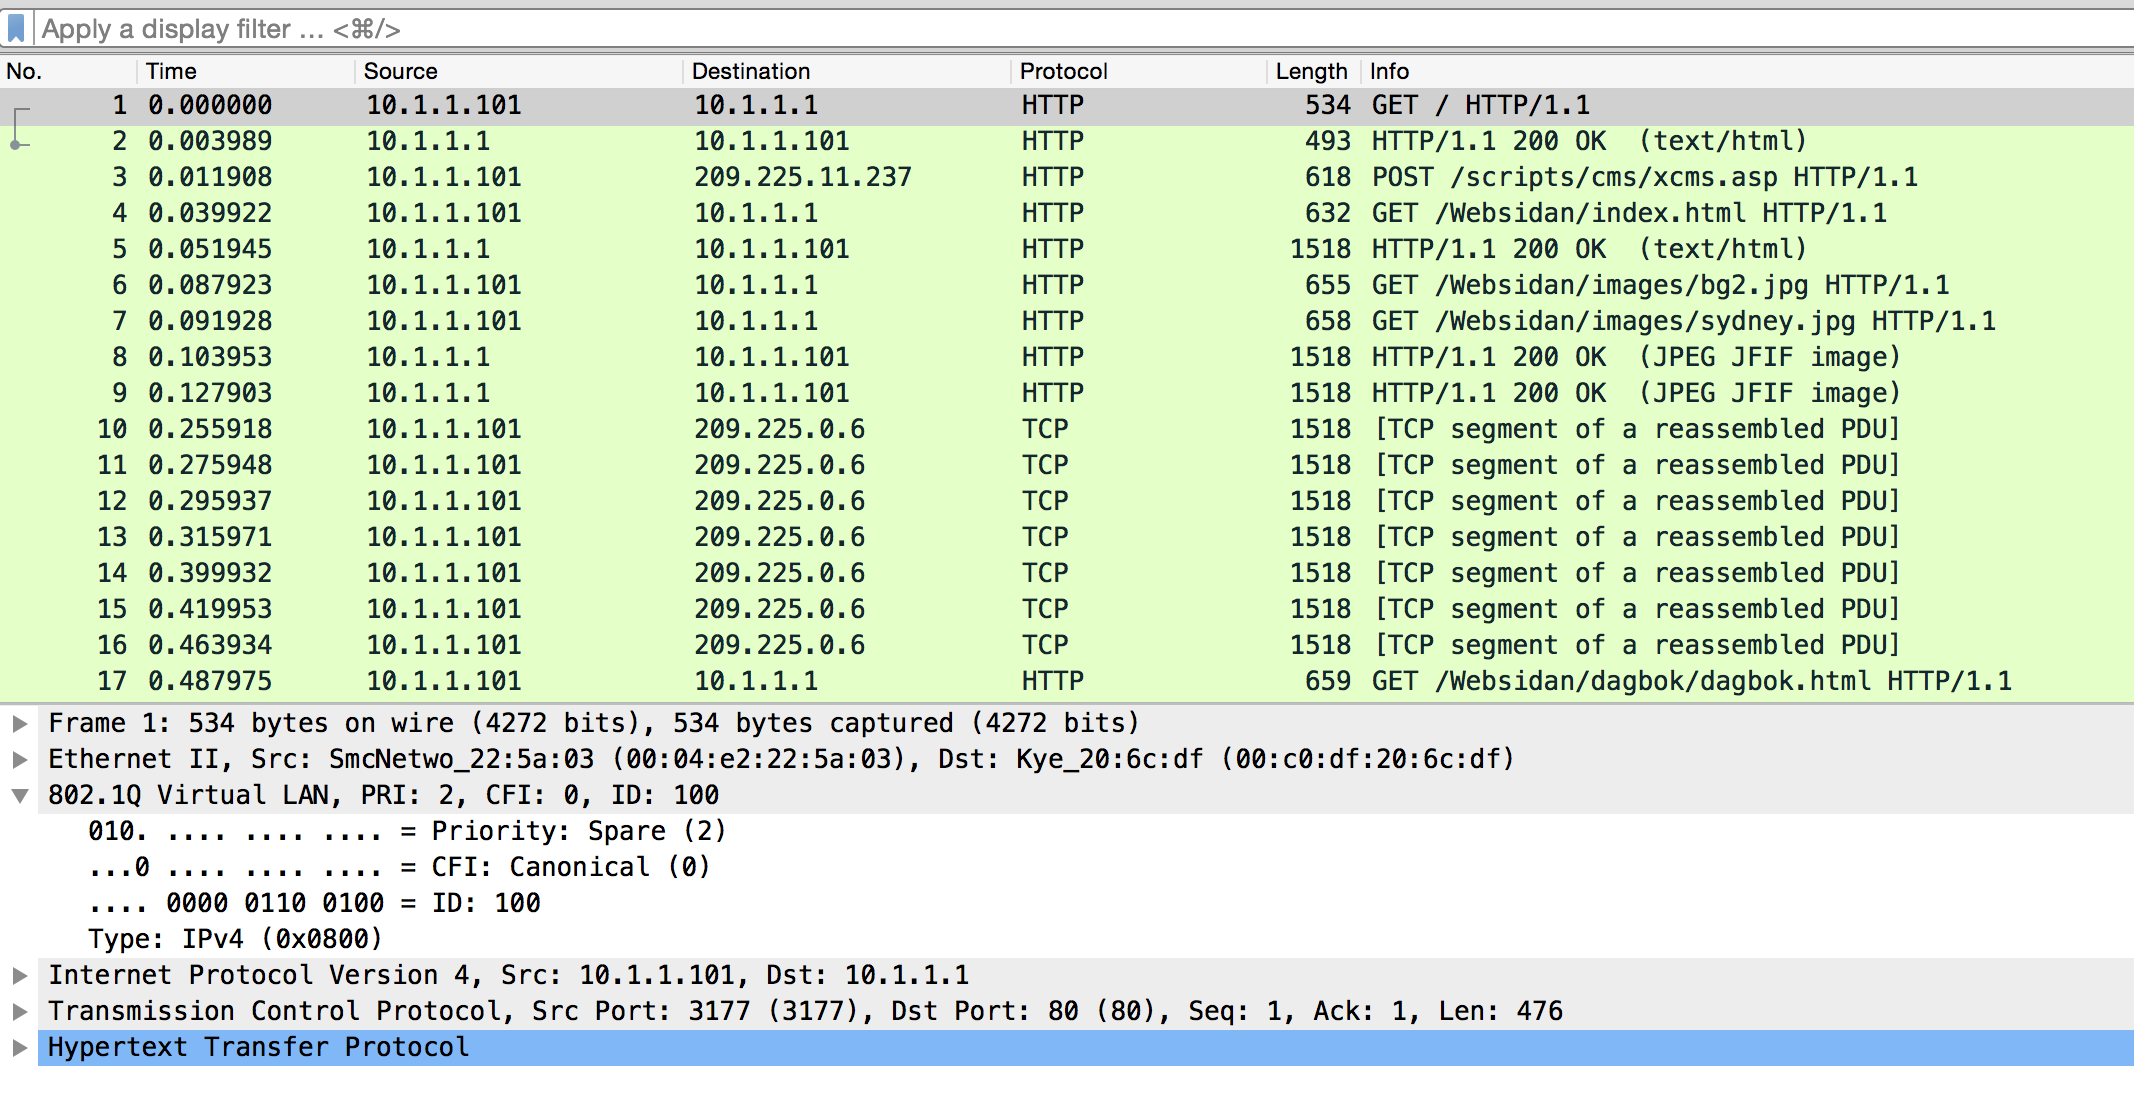
\includegraphics[scale=0.45]{pictures/wireshark}
\caption{Выходной трафик}
\label{pic:wireshark}
\end{figure}

Как видно на рисунке~\ref{pic:wireshark}, к пакету добавилась VLAN метка с содержимым, заданным в конфигурационном файле. Это позволяет сделать вывод о правильности функционирования разработанного сервиса.

\subsection{Нагрузочное тестирование}

\paragraph{Выводы}

В рамках данного раздела производится выбор операционной системы и языка программирования, приводится список дополнительных инструментов, использующихся при разработке, и команды для их установки из репозиториев Ubuntu. Также описываются классы, их назначение в рамках всей системы, и методы, использующиеся в работе сервиса. В конце раздела отражены результаты по каждому виду проведенного в рамках разработки тестирования.
